% 第二章 双目立体视觉理论基础

\chapter{双目立体视觉理论基础}
%------------------------------------------------------------------------------------
\section{摄像机模型}
\subsection{常用坐标系定义及变换}
% ref: 吴哲岑ch2.2,p10; 王德海ch2.1,p9; 王莹ch2.2, p7
% 图像坐标系,摄像机坐标系,世界坐标系
% 图像像素坐标系,图像物理坐标系(成像平面坐标系)
摄像机的成像变换过程涉及到三维的真实世界与二维的图像平面。在视觉测量过程中,世界空间中的点被投影到图像平面上,因此需要定义不同的坐标系并掌握各个坐标系之间的变换方法。常用坐标系包括图像坐标系、成像平面坐标系(也叫图像物理坐标系)、摄像机坐标系和世界坐标系和。

(1)图像坐标系

摄像机采集的图像是以二维(灰度图)或三维(彩色图像)数组的形式储存在计算机中的。设一张图像的分辨率为$M\times N$,则相应得到一个$M\times N$的二维数组,数组中每个元素对应图像中一个像素点。 如图\ref{fig:2_1_image_coord}所示,以图像的左上角为坐标系原点,横轴U指向右、纵轴V指向下,建立直角坐标系$O-UV$,称之为图像坐标系(或图像像素坐标系)。坐标点(u, v)对应图像中第v行第u列的像素。

\begin{figure}[!htb] %图像坐标系和成像平面坐标系
	\centering
	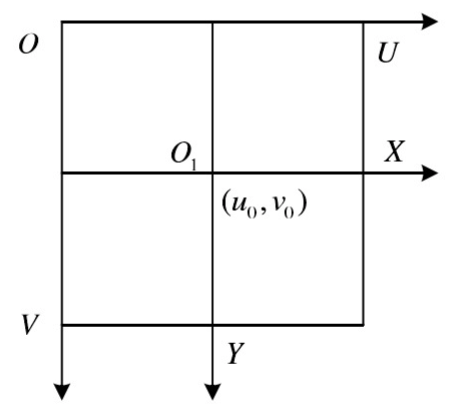
\includegraphics[width=2in]{figures/2_1_image_coord}
	\caption{图像坐标系和成像平面坐标系}\label{fig:2_1_image_coord}
\end{figure}

(2)成像平面坐标系

图像坐标系以像素为基本单位,而现实中以毫米等物理单位来描述物体的尺寸和位置。因此,定义成像平面坐标系$O_1-XY$来建立像素与物理长度之间的联系。在$O_1-XY$坐标系中,定义图像平面与摄像机光轴的交点$O_1$为坐标原点,也称为图像主点。理想情况下,主点位于图像的中心位置,但现实中制造的摄像机会有一定的偏差。坐标轴X、Y轴分别平行于坐标轴U、V。假设主点$O_1$在$O-UV$坐标系中的坐标为$(u_0, v_0)$,每个像素在图像宽和高方向的物理尺寸分别为$d_x$和$d_y$,则图像中某点在成像平面坐标系下的坐标$(x, y)$和图像坐标系下的坐标$(u,v )$之间的关系可表示为:
%
\begin{equation}\label{eq:2_1_image_coord}
\left\{
	\begin{aligned}
	u&=\frac{x}{d_x}+u_0 \\
	v&=\frac{y}{d_y}+v_0 \\
	\end{aligned}
\right.
\end{equation}

为了便于后面的坐标转换,将其表示成齐次坐标的矩阵形式:
\begin{eqnarray}\label{eq:2_1_image_coord_homogeneous}
\left[\begin{array}{c} u \\ v \\ 1 \end{array} \right]
=
\left[\begin{array}{ccc}
\frac{1}{d_x} & 0 & u_0 \\
0 & \frac{1}{d_y} & v_0 \\
0 & 0 & 1
\end{array}
\right]
\hspace{-6pt} %默认的间距有点大,不知道怎么调整。。
\left[\begin{array}{c} x \\ y \\ 1 \end{array}\right]
\end{eqnarray}

(3)摄像机坐标系

沿摄像机光轴方向移动成像平面坐标系,使坐标原点与光心$O_c$重合,定义Z轴垂直于成像平面坐标系,即摄像机的光轴,从而得到摄像机坐标系$O_c-X_cY_cZ_c$,如图\ref{fig:2_1_camera_and_world_coord}所示。摄像机光心$O_c$到成像平面坐标系原点$O_1$的距离$O_c O_1$即为摄像机的焦距$f$。

\begin{figure}[!htb] %图像坐标系和成像平面坐标系
	\centering
	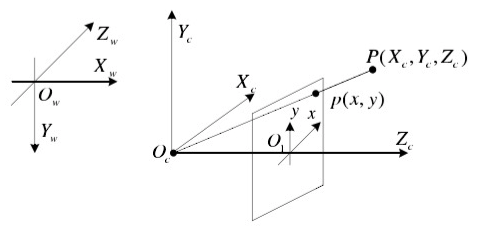
\includegraphics[width=4in]{figures/2_1_camera_and_world_coord}
	\caption{图像坐标系和成像平面坐标系}\label{fig:2_1_camera_and_world_coord}
\end{figure}

(4)世界坐标系

摄像机在三维空间中的位置通常不是固定的,因此更了更方便地描述场景中目标物体的真实位置,需建立一个唯一的世界坐标系$O_w-X_wY_wZ_w$。设场景中任一点在世界坐标系和摄像机坐标系下的坐标分别为$(X_w, Y_w, Z_w)$和$(X_c, Y_c, Z_c)$,则二者之间的转换可以表示为:
%
\begin{eqnarray}\label{eq:2_1_world_camera_coord_transform}
\left[\begin{array}{c} X_c \\ Y_c \\ Z_c \\ 1 \end{array} \right]
=
\left[\begin{array}{cc}
\mathbf{R} & \mathbf{t}  \\
\mathbf{0^T} & 1
\end{array}
\right]
\hspace{-6pt} %默认的间距有点大,不知道怎么调整。。
\left[\begin{array}{c} X_w \\ Y_w \\ Z_w \\ 1 \end{array}\right]
=\mathbf{M_2}
\hspace{-3pt} 
\left[\begin{array}{c} X_w \\ Y_w \\ Z_w \\ 1 \end{array}\right]
\end{eqnarray}
其中,$\mathbf{R}$和$\mathbf{t}$分别用来描述两坐标系之间的旋转和平移关系,$\mathbf{R}$为$3\times 3$的正交矩阵,$\mathbf{t}$为长度为3的向量,$\mathbf{0_t}=[0, 0, 0]$,$\mathbf{M_2}$为$4\times4$的矩阵。


%------------------------------------------------------------------------------------
\subsection{摄像机线性模型}
% ref: 尚倩ch2.1,p13; 王德海ch2.1, p11; 吴哲岑ch3.1,p19; 苏东ch2.1, p10.
摄像机的线性模型即针孔(pinhole)模型\cite{zhang1999flexible, zhang2000flexible}。在此模型中,来自某一点的光线从物体上发射过来,通过一个平面上的针孔,投射在成像平面上,其余的光束都被针孔平面所阻挡,如图\ref{fig:2_1_pinhole_model}所示。因此物体在图像中的大小只需要一个参数来描述:焦距(focal length),即针孔到成像平面的距离。 设摄像机焦距为$f$,相机到所拍物体的距离为$Z_c$,所拍物体的尺寸为$X_c$,则利用三角形相似原理可以得到:
%
\begin{equation}\label{eq:2_1_triangular_similarity}
-x = f \cdot \frac{X_c}{Z_c}
\end{equation}

\begin{figure}[!htb] %摄像机针孔模型
	\centering
	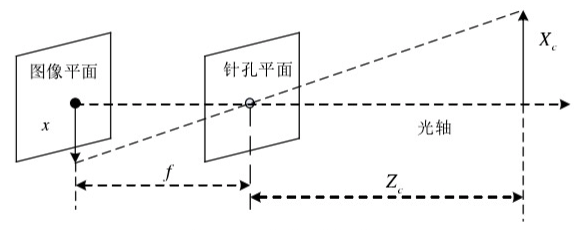
\includegraphics[width=4in]{figures/2_1_pinhole_model}
	\caption{摄像机针孔模型}\label{fig:2_1_pinhole_model}
\end{figure}

% TODO: 差个调整后的针孔模型图
负号的存在表示图像中的物体是倒立的。为了略去等式左侧的负号,我们把图像平面放到针孔的右侧,形成了更直观的三角形相似关系$x/f = X_c/Z_c$,图像中的物体由倒立变为了正立。因此,摄像机坐标系下的点$P(X_c, Y_c, Z_c)$在成像平面上的坐标可表示为
%
\begin{eqnarray}\label{eq:2_1_imaging_plane_and_world_transform}
Z_c
\left[\begin{array}{c} x \\ y \\ 1 \end{array} \right]
=
\left[\begin{array}{cccc}
f & 0 & 0 & 0 \\
0 & f & 0 & 0 \\
0 & 0 & 1 & 0
\end{array}
\right]
\hspace{-6pt} %默认的间距有点大,不知道怎么调整。。
\left[\begin{array}{c} X_c \\ Y_c \\ Z_c \\ 1 \end{array}\right]
\end{eqnarray}

综合式\ref{eq:2_1_image_coord_homogeneous}、\ref{eq:2_1_world_camera_coord_transform}和\ref{eq:2_1_imaging_plane_and_world_transform},可以得到空间中任意一点$P$在世界坐标系和图像坐标系下的坐标转换关系:
%
\begin{eqnarray}\label{eq:2_1_image_and_world_transform}
Z_c
\left[\begin{array}{c} u \\ v \\ 1 \end{array} \right]
=
\left[\begin{array}{ccc}
\frac{1}{d_x} & 0 & u_0 \\
0 & \frac{1}{d_y} & v_0 \\
0 & 0 & 1
\end{array}\right]
\hspace{-6pt}
\left[\begin{array}{cccc}
f & 0 & 0 & 0 \\
0 & f & 0 & 0 \\
0 & 0 & 1 & 0
\end{array}\right]
\hspace{-6pt}
\left[\begin{array}{cc}
\mathbf{R} & \mathbf{t}  \\
\mathbf{0^T} & 1
\end{array}\right]
\hspace{-6pt}
\left[\begin{array}{c} X_w \\ Y_w \\ Z_w \\ 1 \end{array}\right] \nonumber
\\
= 
\left[\begin{array}{cccc}
\alpha_x & 0 & u_0 & 0 \\
0 & \alpha_y & v_0 & 0 \\
0 & 0 & 1 & 0
\end{array}\right]
\hspace{-6pt}
\left[\begin{array}{cc}
\mathbf{R} & \mathbf{t}  \\
\mathbf{0^T} & 1
\end{array}\right]
\hspace{-6pt}
\left[\begin{array}{c} X_w \\ Y_w \\ Z_w \\ 1 \end{array}\right]
=
\mathbf{M_1} \mathbf{M_2}
\left[\begin{array}{c} X_w \\ Y_w \\ Z_w \\ 1 \end{array}\right]
= \mathbf{M}
\left[\begin{array}{c} X_w \\ Y_w \\ Z_w \\ 1 \end{array}\right]
\end{eqnarray}
其中,$\alpha_x=\frac{f}{d_x}$,$\alpha_y=\frac{f}{d_y}$,$\alpha_x, \alpha_y, u_0, v_0$只与摄像机的内部结构有关,为摄像机的内部参数;$\mathbf{R}, \mathbf{t}$描述的是摄像机坐标系与世界坐标系的相对位置关系,为摄像机的外部参数。$\mathbf{M_1}$和$\mathbf{M_2}$分别称为内参矩阵(intrinsic matrix)和外参矩阵(extrinsic matrix)。对于一部摄像机来说,内部参数是固定不变的,而外部参数可能改变。$\mathbf{M}=\mathbf{M_1 M_2}$为$3\times 4$的投影矩阵,摄像机将将三维空间中的点映射到二维投影平面上的过程叫作投影变换。

注意到内参$\alpha_x$实际上是透镜的物理焦距长度$f$与成像尺度因子$s_x=\frac{1}{d_x}$的乘积,这样做的意义在于$f$的单位是mm,$s_x$的单位是像素/mm,从而$\alpha_x$的单位是像素。摄像机的标定并不能得到$f$和$s_x$,只有组合量$\alpha_x$和$\alpha_y$可以通过标定直接计算出来。

%------------------------------------------------------------------------------------
\subsection{摄像机非线性模型}
% ref: 白鹏,尚倩,王德海,吴哲岑.
针孔模型只是一个理想的模型,而实际情况下通过光心的光线太少会导致曝光不足,图像生成缓慢。因此我们生活中使用的摄像机都利用透镜来使足够多的光线收敛聚焦到成像平面上\cite{GaryBradski2009学习}。理论上可以定义不造成任何畸变的透镜,但现实中由于制造工艺问题,所有透镜都存在一定程度的畸变。为了获得较为精确的摄像机模型,需要对畸变进行建模。

摄像机的畸变主要有径向畸变(radial distortions)\cite{hartley2003multiple}、离心畸变(decentering distortions)\cite{ricolfe2010lens}和薄棱镜畸变(thin prism distortions)\cite{weng1992camera}。第一种主要是由棱镜的形状缺陷导致的,其只会造成径向位置误差;后两种主要是由棱镜和相机的不当安装导致的,它们会同时造成径向和切向的位置误差\cite{weng1992camera}。

我们可以使用一组数学表达式来表示畸变,在摄像机的线性模型基础上加入畸变的表达式,得到一个摄像机的非线性模型。非线性畸变可表示为式\ref{eq:2_1_lens_distortion}的形式。
%
\begin{equation}\label{eq:2_1_lens_distortion}
\left\{
\begin{aligned}
x' &= x + \sigma_x (x,y)  \\
y' &= y + \sigma_y(x,y)
\end{aligned}
\right.
\end{equation}
其中,$(x,y)$是线性模型计算得到的成像平面坐标系下的坐标,$(x',y')$是计入畸变后更准确的坐标,$\sigma_x$和$\sigma_y$是非线性模型中的畸变参数。

(1)径向畸变

径向畸变又称径向失真,主要是由棱镜的径向曲率曲线的缺陷造成的。径向畸变可分为两类,符号为负的径向位移被称为桶形畸变(barrel distortion),它会使距离光心远的点挤向一起;符号为正的径向位移被称为枕形畸变(pincushion),它会使距离光心远的点更加分散。这种畸变关于光轴是严格对称的,我们可以用泰勒展开式来对径向畸变建模,如式\ref{eq:2_1_radial_distortion}。试验表明,使用$k1$和$k2$两项即可校正90\%以上的径向畸变\cite{hartley2003multiple}。
%
\begin{equation}\label{eq:2_1_radial_distortion}
\left\{
\begin{aligned}
\sigma_x(x,y) &= x(k_1 r^2 + k_2 r^4 + k_3 r^6 + \cdots)  \\
\sigma_y(x,y) &= y(k_1 r^2 + k_2 r^4 + k_3 r^6 + \cdots) 
\end{aligned}
\right.
\end{equation}

\begin{figure}[!htb] %桶形畸变和枕形畸变
	\centering
	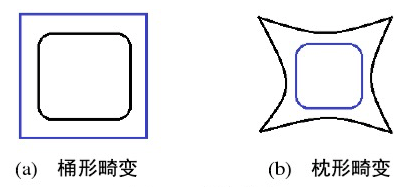
\includegraphics[width=4in]{figures/2_1_radial_distortion}
	\caption{桶形畸变和枕形畸变系}\label{fig:2_1_radial_distortion}
\end{figure}

(2)离心畸变

离心畸变是镜头各部件的光心不严格共线造成的,现实中的光学系统都存在不同程度的离心畸变。这种畸变可描述为式\ref{eq:2_1_decentering_distortion}。
%
\begin{equation}\label{eq:2_1_decentering_distortion}
\left\{
\begin{aligned}
\sigma_x(x,y) &= 2p_2 xy + p_1 (3x^2 + y^2)  \\
\sigma_y(x,y) &= 2p_1 xy + p_2 (x^2+ 3y^2)
\end{aligned}
\right.
\end{equation}

(3)薄棱镜畸变

薄棱镜畸变是由透镜的设计、生产和相机装配中的缺陷造成的,例如透镜光轴与摄像机的面阵平面之间存在微小的倾斜。这种畸变可使用式\ref{eq:2_1_thin_prism_distortion}来表示。
%
\begin{equation}\label{eq:2_1_thin_prism_distortion}
\left\{
\begin{aligned}
\sigma_x(x,y) &= s_1 (x^2 + y^2) \\
\sigma_y(x,y) &= s_2 (x^2 + y^2)
\end{aligned}
\right.
\end{equation}

三种畸变中,径向畸变是最主要的畸变成分,薄棱镜畸变的影响很小,可忽略不计。因此,综合径向畸变和离心畸变,透镜畸变模型可表示为:
%
\begin{equation}\label{eq:2_1_overall_distortion}
\left\{
\begin{aligned}
\sigma_x(x,y) &= x(k_1 r^2 + k_2 r^4) + (2p_2 xy + p_1 (3x^2 + y^2))  \\
\sigma_y(x,y) &= y(k_1 r^2 + k_2 r^4)  + (2p_1 xy + p_2 (x^2 + 3y^2))
\end{aligned}
\right.
\end{equation}


%------------------------------------------------------------------------------------
\section{摄像机标定}
% ref: 王德海,时洪光,尚倩, 吴哲岑,王莹
摄像机标定就是确定其内部参数和外部参数的过程。对于双目摄像机,标定分为两步:首先分别标定两个相机得到其内部参数,然后再求解它们之间的相对位置关系,即旋转矩阵和平移向量。

\subsection{单目摄像机标定}
摄像机标定方法主要可分为传统标定方法和自标定方法。传统标定方法\cite{李小平2008双目视觉立体测量研究}又称为强标定,一般需要在摄像机前放置一个标定参照物,摄像机拍摄标定物后获得标定物上特征点在图像上的坐标,同时在世界坐标系下测量标定物特征点的坐标,利用图像坐标系下和世界坐标系下坐标的对应关系,借助非线性优化方法计算摄像机的内外参数\cite{时洪光2010基于双目视觉的运动目标定位研究}。自标定方法\cite{李洪海2007摄像机标定技术研究}由Faugerasa等人提出,仅利用图像间成像点的对应关系就可以得到摄像机参数\cite{王德海2016基于双目立体视觉的目标识别与抓取定位}。

传统标定方法标定精度较高,但计算复杂且需要标定模板;自标定方法操作简便灵活,但鲁棒性差、精度低。张正友于1999年提出了一种介于传统标定和自标定方法之间的新方法\cite{zhang1999flexible},只需要一个平面的标定板,操作简单,鲁棒性好,精度较高,近年来被广泛应用。本文使用这种方法进行摄像机的标定。

张正友标定法的基本思想是:摄像机的外部参数变化而内部参数恒定,使用一个确定规格的标定板从不同角度进行拍摄,每张图像可以用来确定一个单应性(Homography),能提供8个方程,同时引入了6个未知量(三维空间的旋转和平移),故得到2个约束条件。使用多张图片即可求解所有内参值。具体算法原理如下。

%(1)建立摄像机的几何模型

设空间中任一点$\mathbf{P}$在图像坐标系和世界坐标系下的坐标分别为$\mathbf{m}=[u,v]^T$和$\mathbf{M}=[X, Y, Z]^T$,齐次坐标形式为$\tilde{\mathbf{m}} = [u,v,1]^T$和$\tilde{\mathbf{M}} = [X,Y,Z,1]^T$。对于线性模型,二者具有如下关系:
%
\begin{equation}\label{eq:2_2_mono_calib_0}
s \tilde{\mathbf{m}} = \mathbf{A} [ \mathbf{R}  \quad  \mathbf{t} ] \tilde{\mathbf{M}}
\end{equation}
其中,$s$为尺度因子,$\mathbf{R}$和$\mathbf{t}$为摄像机的外参,$\mathbf{A}$为摄像机内参矩阵。相较上一节中建立的线性模型,Zhang\cite{zhang2000flexible}在模型中多考虑了相机两个轴之间的倾斜,因此$\mathbf{A}$表示为:
%
\begin{equation}\label{eq:2_2_mono_calib_1}
\mathbf{A}=
\left[ \begin{array}{ccc}
\alpha_x & \gamma & u_0 \\
0 & \alpha_y & v_0 \\
0 & 0 & 1
\end{array} \right]
\end{equation}
$\gamma$描述相机两个轴之间非严格正交所造成的影响,其余参数的定义与上一节线性模型中的定义相同。
为了简化问题,我们假定标定板图像所在平面与世界坐标系中$X_wOY_w$平面重合,故所有点的坐标$Z=0$。使用$\mathbf{r_i}$表示矩阵$\mathbf{R}$的第$i$列,则式\ref{eq:2_2_mono_calib_0}可简化为:
%
\begin{equation}\label{eq:2_2_mono_calib_2}
s
\begin{bmatrix}
u \\ v \\ 1
\end{bmatrix}
= \mathbf{A} \hspace{2pt}  [ \mathbf{r_1} \quad \mathbf{r_2} \quad \mathbf{r_3} \quad \mathbf{t} ]
\begin{bmatrix}
X \\ Y \\ 0 \\ 1
\end{bmatrix}
= \mathbf{A} \hspace{2pt}  [ \mathbf{r_1} \quad\mathbf{r_2} \quad \mathbf{t} ]
\begin{bmatrix}
X \\ Y \\ 1
\end{bmatrix}
\end{equation}

从而,点$\mathbf{P}$在两个坐标系下的坐标变换可以用单应性矩阵$\mathbf{H}$来表示:
%
\begin{equation}\label{eq:2_2_mono_calib_3}
s \tilde{\mathbf{m}} = \mathbf{H} \tilde{\mathbf{M}}
\end{equation}
其中,$\mathbf{H} = \mathbf{A} [ \mathbf{r_1} \quad \mathbf{r_2} \quad \mathbf{t} ]$是$3\times 3$的矩阵。令$\mathbf{H} = [\mathbf{h_1}, \mathbf{h_2}, \mathbf{h_3}]$,那么
%
\begin{equation}\label{eq:2_2_mono_calib_4}
[\mathbf{h_1} \quad \mathbf{h_2} \quad \mathbf{h_3}]
= \lambda \mathbf{A} [ \mathbf{r_1} \quad \mathbf{r_2} \quad \mathbf{t} ]
\end{equation}
$\lambda$是一个常数。由于$\mathbf{R}$是正交矩阵,其列向量$\mathbf{r_1}$与$\mathbf{r_2}$相互正交,故有
%
\begin{equation}\label{eq:2_2_mono_calib_5}
\left\{
\begin{aligned}
\mathbf{h}_1^T\mathbf{A}^{-T}\mathbf{A}^{-1}\mathbf{h}_2 &= 0 \\
 \mathbf{h}_1^T\mathbf{A}^{-T}\mathbf{A}^{-1}\mathbf{h}_1 &= \mathbf{h}_2^T\mathbf{A}^{-T}\mathbf{A}^{-1}\mathbf{h}_2 
\end{aligned}
\right.
\end{equation}
式\ref{eq:2_2_mono_calib_5}表示的是一个单应性对摄像机内部参数施加的两个约束。单应性矩阵有8个自由度,但额外引入了6个外部参数(三维空间的旋转和平移),因此只能得到两个约束条件。要求解所有的内部参数,需要使用多个单应性的信息。

令
%
\begin{equation}\label{eq:2_2_mono_calib_6}
\begin{split}
\mathbf{B} = \mathbf{A}^{-T} \mathbf{A}^{-1} \equiv
\begin{bmatrix}
B_{11} & B_{12} & B_{13} \\
B_{21} & B_{22} & B_{23} \\
B_{31} & B_{32} & B_{33} \\
\end{bmatrix} \hspace{1.5in}
\\
=
\begin{bmatrix}
	\frac{1}{\alpha_x^2} &
	 -\frac{\gamma}{\alpha_x^2 \alpha_y} &
	 \frac{v_0\gamma - u_0 \alpha_y}{\alpha_x^2 \alpha_y} \\
	-\frac{\gamma}{\alpha_x^2 \alpha_y} &
	 \frac{\gamma^2}{\alpha_x^2 \alpha_y^2} + \frac{1}{\alpha_y^2} &
	  -\frac{\gamma(v_0 \gamma - u_0 \alpha_y)}{\alpha_x^2 \alpha_y^2} - \frac{v_0}{\alpha_y^2} \\
	\frac{v_0 \gamma - u_0 \alpha_y}{\alpha_x^2 \alpha_y} &
	 -\frac{\gamma (v_0 \gamma - u_0 \alpha_y)}{\alpha_x^2 \alpha_y^2} - \frac{v_0}{\alpha_y^2} &
	 \frac{ (v_0 \gamma - u_0 \alpha_y)^2 }{\alpha_x^2 \alpha_y^2} + \frac{v_0^2}{\alpha_y^2} + 1
\end{bmatrix}
\end{split}
\end{equation}
注意到$\mathbf{B}$是对称阵,可以定义一个6维向量来表示:
%
\begin{equation}\label{eq:2_2_mono_calib_7}
\mathbf{b} = [B_{11}, B_{12}, B_{22}, B_{13}, B_{23}, B_{33}]^T
\end{equation}

令$\mathbf{H}$的第$i$列为$\mathbf{h_i} = [h_{i1}, h_{i2}, h_{i3}]^T$,则有
%
\begin{equation}\label{eq:2_2_mono_calib_8}
\mathbf{h}_I^T \mathbf{B} \mathbf{h}_j = \mathbf{v}_{ij}^T \mathbf{b}
\end{equation}
其中,$\mathbf{v}_{ij} = [h_{i1} h_{j1}, h_{i2} h_{j2} + h_{i2} h_{j1}, h_{i2} h_{j2}, h_{i3} h_{j1} +h_{i1} h_{j3}, h_{i3} h_{j2} + h_{i2} h_{j3}, h_{i3} h_{j3}]^T$。
从而两个约束方程\ref{eq:2_2_mono_calib_5}可以改写为$\mathbf{b}$的齐次方程组:
%
\begin{equation}\label{eq:2_2_mono_calib_9}
\begin{bmatrix}
\mathbf{v}_{12}^T \\ (\mathbf{v}_{11} - \mathbf{v}_{22})^T
\end{bmatrix}
\mathbf{b} = \mathbf{0}
\end{equation}

对标定板的$n$幅图片,则联立$n$个方程组\ref{eq:2_2_mono_calib_9}为
%
\begin{equation}\label{eq:2_2_mono_calib_10}
\mathbf{Vb} = \mathbf{0}
\end{equation}
$\mathbf{V}$是一个$2n \times 6$的矩阵。如果$n \geq 3$,我们可以得到$\mathbf{b}$的唯一解;如果$n = 2$,我们可以令$\gamma=0$,从而得到唯一解;如果$n=1$,则我们只能假设一部分内参数已知来求解另外2个内参数。方程组\ref{eq:2_2_mono_calib_10}的解是$\mathbf{V}^T\mathbf{V}$最小特征值对应的特征向量。

在求得$\mathbf{b}$之后,即可通过以下公式来计算摄像机所有的内部参数:
%
\begin{equation}\label{eq:2_2_mono_calib_11}
	\left\{ 
	\begin{aligned}
		v_0 &= (B_{12}B_{13}-B_{11}B_{23}) / (B_{11}B_{22} - B_{12}^2) \\
		\lambda &= B_{33} - [B_{13}^2 + v_0 (B_{12}B_{13} - B_{11}B_{23})] / B_{11} \\
		\alpha_x &= \sqrt{\lambda / B_{11}} \\
		\alpha_y &= \sqrt{\lambda B_{11} / (B_{11}B_{22} - B_{12}^2)} \\
		\gamma &= -B_{12}\alpha_x^2 \alpha_y / \lambda \\
		u_0 &= \gamma v_0 / \alpha_x - B_{13} \alpha_x^2 / \lambda
	\end{aligned}
	\right.
\end{equation}

得到$\mathbf{A}$后即可利用下式计算外部参数:
%
\begin{equation}\label{eq:2_2_mono_calib_12}
	\mathbf{r}_1 = \lambda \mathbf{A}^{-1}\mathbf{h}_1, \quad
	\mathbf{r}_2 = \lambda \mathbf{A}^{-1}\mathbf{h}_2, \quad
	\mathbf{r}_3 = \mathbf{r}_1 \times \mathbf{r}_2, \quad
	\mathbf{t} = \lambda \mathbf{A}^{-1}\mathbf{h}_3
\end{equation}
$\lambda = 1/||\mathbf{A}^{-1}\mathbf{h}_1||$。一般计算得到的矩阵$\mathbf{R}$并不满足旋转矩阵的性质,可以使用奇异值分解等方法获得更好的解。

由于拍摄图片中存在噪声,提取的角点会存在误差,可以通过最小化式\ref{eq:2_2_mono_calib_13}中的目标函数来得到各角点坐标的最大似然估计:
%
\begin{equation}\label{eq:2_2_mono_calib_13}
\sum_{i=1}^{n} \sum_{j=1}^{m}|| \mathbf{m}_{ij} - \hat{\mathbf{m}}(\mathbf{A}, \mathbf{R}_i, \mathbf{t}_i, \mathbf{M}_j) ||^2
\end{equation}
式中,$\hat{\mathbf{m}}(\mathbf{A}, \mathbf{R}_i, \mathbf{t}_i, \mathbf{M}_j)$表示点$\mathbf{M}_j$在图像$i$中的投影。该非线性最小化问题可利用Levenberg-Marquardt算法迭代求解,使用前面的结果作为初值。优化时中可以加入畸变项以得到畸变参数。

%------------------------------------------------------------------------------------
\subsection{双目摄像机标定}
% ref: 王德海,王莹,邓国栋,时洪光. 都是一样的公式。
双目摄像机标定是在完成两个单目摄像机标定的基础上,求解它们之间的旋转矩阵$R$和平移向量$t$的过程。
设左右相机的外部参数分别为$(\mathbf{R}_1, \mathbf{t}_1)$和$(\mathbf{R}_2, \mathbf{t}_2)$,世界坐标系下某点$\mathbf{x}_w$在两个摄像机坐标系下的分别表示为$\mathbf{x}_l$和$\mathbf{x}_r$,则
%
\begin{equation}\label{eq:2_2_binono_calib_0}
\mathbf{x}_l = \mathbf{R}_l + \mathbf{t}_l, \quad \mathbf{x}_r = \mathbf{R}_r + \mathbf{t}_r
\end{equation}

联立两式,消去$\mathbf{x}_w$,得到$\mathbf{x}_l$和$\mathbf{x}_r$的关系为
%
\begin{equation}\label{eq:2_2_binono_calib_1}
\mathbf{x}_r = \mathbf{R}_r \mathbf{R}_l^{-1}\mathbf{x}_l +
 ( \mathbf{t}_r - \mathbf{R}_r \mathbf{R}_l^{-1}\mathbf{t}_l )
\end{equation}

从而可知两摄像机之间的旋转和平移关系分别为
%
\begin{equation}\label{eq:2_2_binono_calib_2}
\mathbf{R} = \mathbf{R}_r \mathbf{R}_l^{-1},  \quad
\mathbf{t} =  \mathbf{t}_r -  \mathbf{R}_r  \mathbf{R}_l^{-1} t_l
\end{equation}

%------------------------------------------------------------------------------------
\subsection{标定结果}
实验使用的摄像机为ZED双目相机,分辨率设置为720p($1280\times 720$)。标定板上的图案为棋盘格,每个方格的边长为$10cm$,共有$7 \times 6$个方格,故每行有6个角点,每列有5个角点。使用ZED相机在室外采集了31组图片,部分标定图像如图\ref{fig:2_2_calib_imgs}所示。

\begin{figure}[!htb] %部分标定图片
	\centering
	\begin{minipage}[c]{0.48\textwidth}
		\centering
		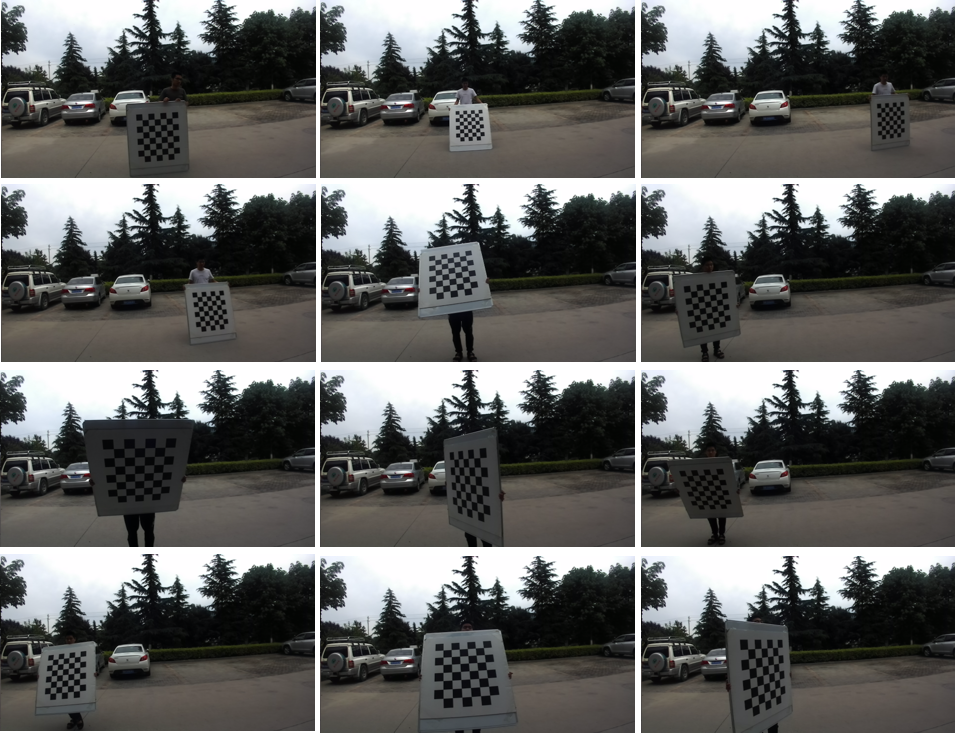
\includegraphics[width=3in]{figures/2_2_calib/left_4x3}
		\centerline{\small{左摄像机采集图片}}
	\end{minipage}
	\hfill
	\begin{minipage}[c]{0.48\textwidth}
		\centering
		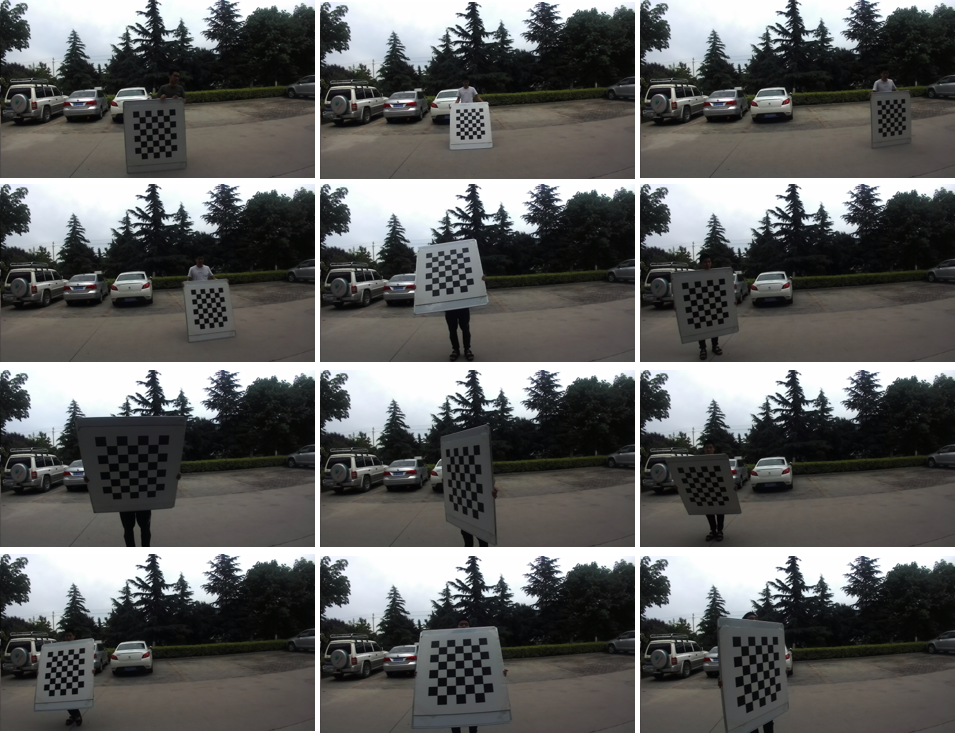
\includegraphics[width=3in]{figures/2_2_calib/right_4x3}
		\centerline{\small{右摄像机采集图片}}
	\end{minipage}
	\caption{部分标定图片}\label{fig:2_2_calib_imgs}
\end{figure}

 分别使用基于OpenCV 2.4.13编写的C++程序和MATLAB双目相机标定工具箱进行了标定操作。经过多次试验,发现OpenCV标定的结果中畸变参数变化很大,结果并不可靠,故在此只给出使用Matlab标定工具箱得到的结果。由于采集图像时光线较暗,标定工具箱共接受了31组图片中的15组,标定结果如表\ref{tab:2_2_calib_result}所示,平均重投影误差(mean reprojection error)为$0.1262$, 各组图片的重投影误差情况见图\ref{fig:2_2_reprojection_errors}。
 
 \begin{table}[!htb] %ZED双目相机标定结果
	\centering
 	\caption{ZED双目相机标定结果}\label{tab:2_2_calib_result}
 	\begin{small}
 	\begin{tabular}{ccc|c} \toprule[2pt]
 		内参数                  & 左相机          & 右相机 & 外参数 \\ \midrule[1pt]
 		$\alpha_x$         & 701.9830   & 703.6765  &
 		\multirow{4}*{$ \mathbf{R} = \left[ \begin{tabular}{ccc}
 			0.9999 & -1.8511e-04 & -0.0108 \\
 			6.8373e-05 & 0.9999 & -0.0108 \\
 			0.0108 & 0.0108 & 0.9999 \end{tabular} \right] $}\\
 		$\alpha_y$         & 701.7472    & 703.3212 & \\
 		$u_0$                  & 604.6113   & 618.4235 & \\
 		$v_0$                  & 366.4776  & 346.8419 & \\
 		畸变系数$k_1$   & -0.1603     & -0.1648 &
 		 \multirow{2}*{$\mathbf{t}=[-120.1123 \quad 0.1007 \quad 2.0492]^T$} \\
 		畸变系数$k_2$   & 0.0138       & 0.0174 & \\ \bottomrule[2pt]
 	\end{tabular}
 	\end{small}
 \end{table}

\begin{figure}[!htb] %标定重投影误差
	\centering
	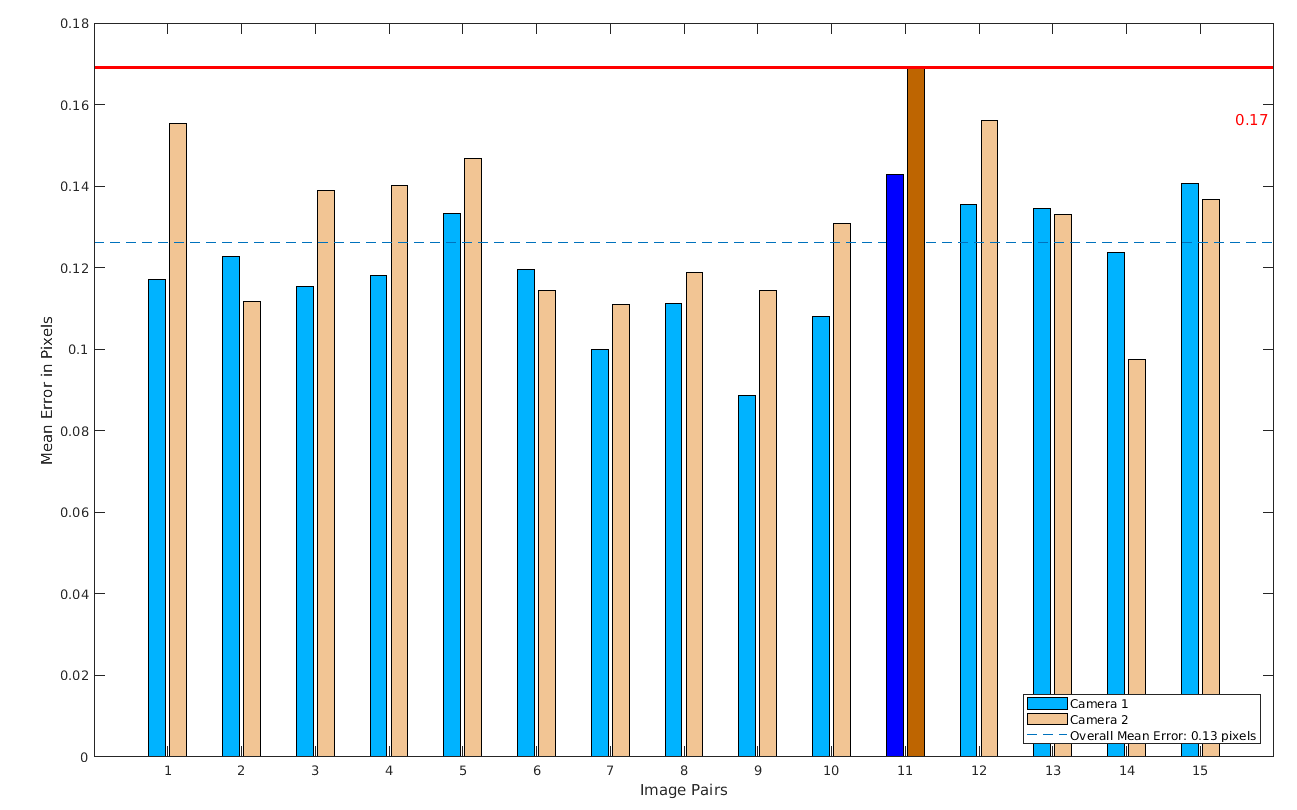
\includegraphics[width=5in]{figures/2_2_reprojection_errors}
	\caption{重投影误差}\label{fig:2_2_reprojection_errors}
\end{figure}

\begin{figure}[!htb] %标定图像的三维位置
		\centering
		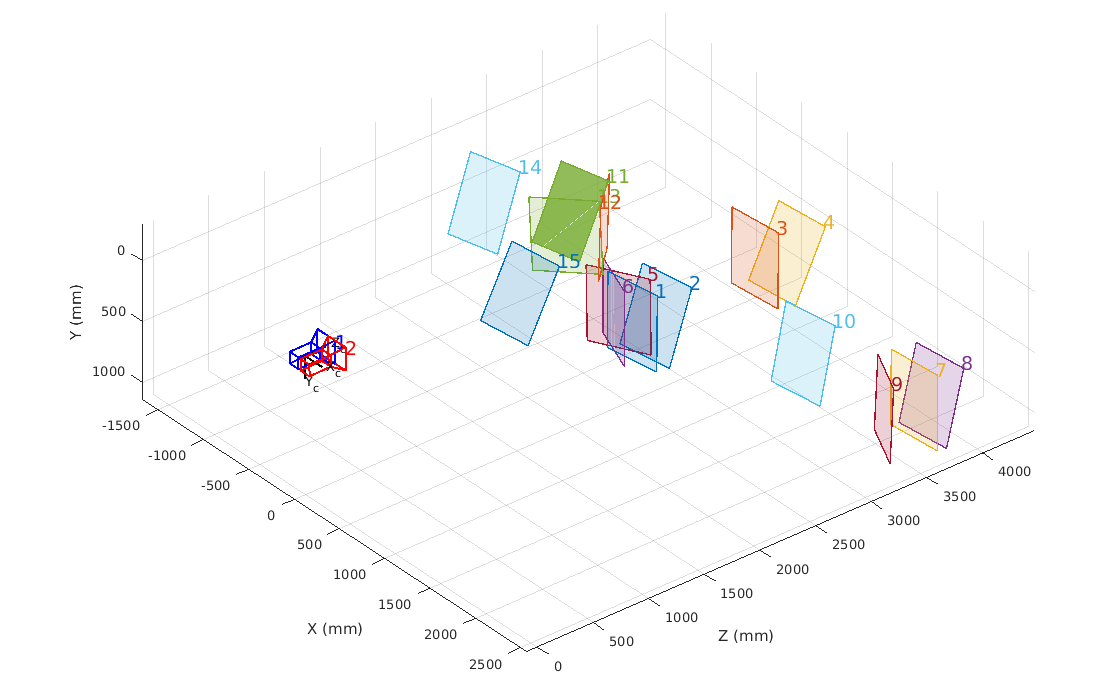
\includegraphics[width=5in]{figures/2_2_extrinsics}
		\caption{标定图像的三维位置}\label{fig:2_2_extrinsics}
\end{figure}

 
%------------------------------------------------------------------------------------
\section{双目立体视觉原理}

\subsection{立体视觉测量原理} % 视差原理
% ref:王莹ch2.3,p16;尚倩ch4.2,p65;陈拓ch2.1,p20.
一个摄像机将三维空间中的点投影到二维平面上,丢失了一些空间信息。如图\ref{fig:2_3_stereo_principle}所示,假设空间中一点$P$在摄像机$C_1$拍摄的图像上为$P_1$,我们并不能根据$P_1$确定$P$的位置,因为由$O_1$和$P_1$确定的直线上的无数个点在图像上的投影都是$P_1$。而如果同时使用两台摄像机$C_1$、$C_2$来观察$P$点,$P$在两张图像上分别为$P_1$、$P_2$,则可以知道$P$同时位于$O_1P_1$和$O_2P_2$两条直线上,故它们的交点就是点$P$在三维空间中的真实位置。

\begin{figure}[!htb] %立体视觉原理
	\centering
	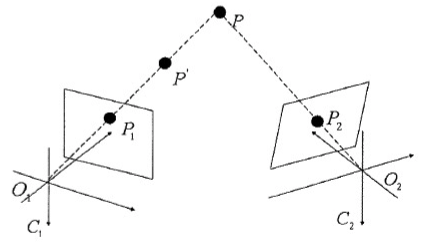
\includegraphics[width=4in]{figures/2_3_stereo_principle}
	\caption{立体视觉原理}\label{fig:2_3_stereo_principle}
\end{figure}

设$P_1$和$P_2$的像素坐标分别为$(u_1, v_1)$和$(u_2, v_2)$,世界坐标系下$P$的坐标是$(X, Y, Z)$,摄像机$C_1$、$C_2$的投影矩阵分别为$M_1$和$M_2$,则有:
%
\begin{equation}\label{eq:2_3_0}
Z_{c1}
\begin{bmatrix}
u_1 \\ v_1 \\ 1
\end{bmatrix}
=
\begin{bmatrix}
m_{11}^1 & m_{12}^1 & m_{13}^1 & m_{14}^1 \\
m_{21}^1 & m_{22}^1 & m_{23}^1 & m_{24}^1 \\
m_{31}^1 & m_{32}^1 & m_{33}^1 & m_{34}^1 \\
\end{bmatrix}
\begin{bmatrix}
X \\ Y \\ Z \\ 1
\end{bmatrix}
\end{equation}

\begin{equation}\label{eq:2_3_1}
Z_{c2}
\begin{bmatrix}
u_2 \\ v_2 \\ 1
\end{bmatrix}
=
\begin{bmatrix}
m_{11}^2 & m_{12}^2 & m_{13}^2 & m_{14}^2 \\
m_{21}^2 & m_{22}^2 & m_{23}^2 & m_{24}^2 \\
m_{31}^2 & m_{32}^2 & m_{33}^2 & m_{34}^2 \\
\end{bmatrix}
\begin{bmatrix}
X \\ Y \\ Z \\ 1
\end{bmatrix}
\end{equation}
$Z_{c1}$、$Z_{c2}$分别为点$P$在两摄像机坐标系下的Z轴坐标。分别消去两式中的$Z_{c1}$和$Z_{c2}$,可以得到$O_1P_1$、$O_2P_2$确定的两条直线的方程:
%
\begin{equation}\label{eq:2_3_2}
\begin{cases}
(u_1 m_{31}^1 - m_{11}^1) X + (u_1 m_{32}^1 - m_{12}^1) Y + (u_1 m_{33}^1 - m_{13}^1) Z = m_{14}^1 - u_1 m_{34}^1 \\
(v_1 m_{31}^1 - m_{21}^1) X + (v_1 m_{32}^1 - m_{22}^1) Y + (v_1 m_{33}^1 - m_{23}^1) Z = m_{24}^1 - v_1 m_{34}^1
\end{cases}
\end{equation}
\begin{equation}\label{eq:2_3_3}
\begin{cases}
(u_2 m_{31}^2 - m_{11}^2) X + (u_2 m_{32}^2 - m_{12}^2) Y + (u_2 m_{33}^2 - m_{13}^2) Z = m_{14}^2 - u_2 m_{34}^2 \\
(v_2 m_{31}^2 - m_{21}^2) X + (v_2 m_{32}^2 - m_{22}^2) Y + (v_2 m_{33}^2 - m_{23}^2) Z = m_{24}^2 - v_2 m_{34}^2
\end{cases}
\end{equation}

联立两式,即可求解点$P$的三维坐标$(X, Y, Z)$。

%------------------------------------------------------------------------------------
\subsection{平行光轴视觉模型与三角测量}
% ref: 王莹ch2.4,p10; 陈拓ch2.1.3,p11; 王德海ch2.4,p27; 吴哲岑ch2.1,p17.
% 学习opencv.
上一小节给出了根据两张图像上的一组对应点来求解该点在三维空间中的位置的基本原理,其对于两个摄像机之间的相对位置并没有任何要求。实际上,通过约束两个摄像机之间的位置,可以将问题简化到二维平面上,从而大大降低计算量。

图\ref{fig:2_3_parallel_optical_axis_model}给出了平行光轴视觉模型。假设两个摄像机是无畸变且相互对准的,其像平面位于同一平面内,光轴严格平行,焦距相同,并且主点在左右图像上具有相同的像素坐标,故两摄像机坐标系的x轴重合,y轴相互平行。称两光心之间的距离为基线距,记为$B$。

\begin{figure}[!htb] %平行光轴视觉模型, 三角测量
	\centering
	\begin{minipage}[c]{0.48\textwidth}
		\centering
		\vspace{0.8in} % 与右图对齐标题
		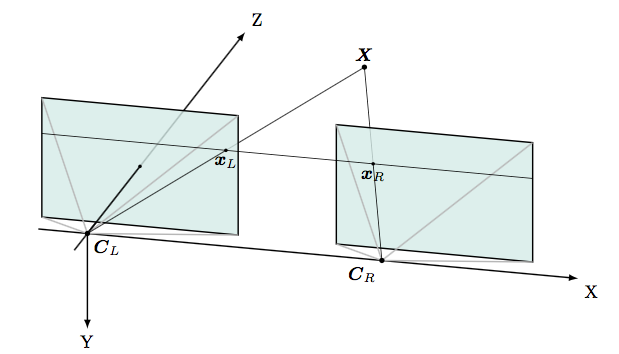
\includegraphics[width=3in]{figures/2_3_parallel_optical_axis_model}
		\caption{平行光轴视觉模型}\label{fig:2_3_parallel_optical_axis_model}
	\end{minipage}
	\hfill
	\begin{minipage}[c]{0.48\textwidth}
		\centering
		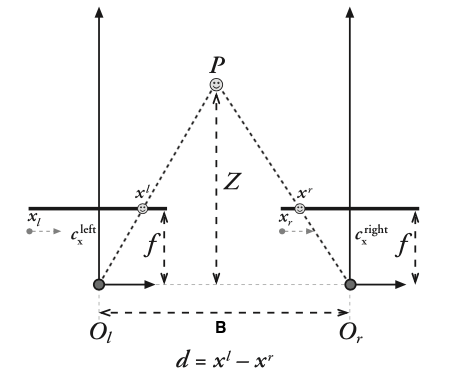
\includegraphics[width=3in]{figures/2_3_triangulation}
		\caption{三角测量}\label{fig:2_3_triangulation}
	\end{minipage}
\end{figure}

设三维空间中的点$P$在左右成像平面上分别为$p_l$和$p_r$,其横坐标分别为$x_l$和$x_r$。由图\ref{fig:2_3_triangulation}易知存在三角形相似关系:
%
\begin{equation}\label{eq:2_3_4}
\frac{B - (x_l - x_r)}{B} = \frac{Z-f}{Z}
\end{equation}
从而有
\begin{equation}\label{eq:2_3_5}
Z = \frac{fB}{x_l - x_r} = \frac{fB}{d}
\end{equation}
称$d=x_l - x_r$为视差(disparity)。由式\ref{eq:2_3_5}可知,在焦距$f$和基线距$B$确定的情况下,空间中任一点$P$的深度$Z$仅与视差$d$有关,且与视差$d$成反比。当视差较大时,视差的微小变化并不会导致深度的显著变化;而当视差趋向0时,微小的视差变化会导致很大的深度变化。因此,双目立体视觉系统仅在一定距离范围内能获得较高的精度。由于使用了三角形相似原理,由视差计算深度的过程被称为三角测量。
% TODO: 实际上因为焦距f是不能通过标定得到的,且视差是在图像坐标系O-UV下定义的(单位是像素),所以这里x_l应该用u_l - u_0来表示,f是alpha_x !!!
(需要说明的是,实际中视差定义在图像坐标系下,其单位为像素,因为上一节中摄像机线性模型处提到过摄像机的焦距$f$是不能通过标定得到的,故实际计算中应使用摄像机线性模型中的$\alpha_x$和像素坐标$u_x-u_0$替代此处公式里的物理焦距$f$和摄像机坐标系下的坐标$x_l$、$x_r$。)


\begin{figure}[!htb] %深度与视差的负相关关系
	\centering
	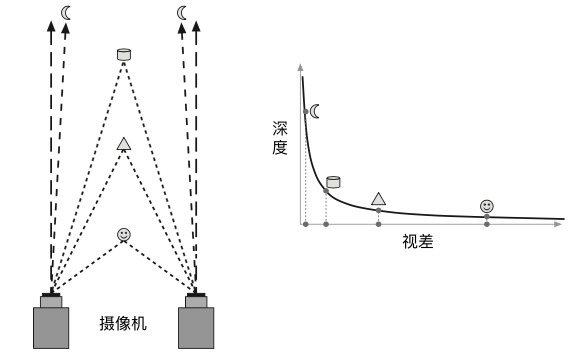
\includegraphics[width=4in]{figures/2_3_depth_vs_disparity}
	\caption{深度与视差的负相关关系}\label{fig:2_3_depth_vs_disparity}
\end{figure}

% TODO: 求X,Y要不要放到第五章的目标定位部分??
类似地,点$P$的$X$、$Y$坐标也满足一定的三角形相似关系,根据下式即可得到点$P$在左摄像机坐标系下的三维坐标:
%
\begin{equation}\label{eq:2_3_6}
\begin{cases}
X_c = \frac{B\cdot x_l }{d} \\
Y_c = \frac{B\cdot y_l }{d} \\
Z_c = \frac{B\cdot f}{d}
\end{cases}
\end{equation}


%------------------------------------------------------------------------------------
\subsection{对极几何}
% ref: 白鹏ch2.2.3, p25; 邓国栋,ch2.5,p25; 陈拓,ch2.1.2,p21. 学习opencv.
%在掌握了由视差计算深度的方法后,另一个需要解决的问题是,如何匹配左右图中的对应点?通常的方法是,在参考图像上选择一个特征点,然后计算其在目标图像上的对应点,一般需要在图像上一定范围内进行逐像素的搜索,选取相似度最高的点作为匹配点。

为了减小立体匹配的搜索范围,提高匹配的效率和准确度,研究人员提出了一系列约束条件:极线约束、相似性约束、唯一性约束、视差连续性约束、顺序单调性约束、左右一致性约束等\cite{陈拓2017CCNN}。其中最重要的一条是极线约束。

对极几何(epipolar geometry)是立体视觉的基本几何学,其描述了三维空间下的几何实体与其在一对摄像机成像平面上的二维投影之间的关系\cite{kowalczuk2015robust}。结合图\ref{fig:2_3_epipolar_geometry},给出对极几何中的几个基本概念:

\begin{itemize}
	\item 基线(baseline):左右摄像机投影中心的连线$O_lO_r$;
	\item 极点(epipole):基线$O_lO_r$与两个成像平面的交点$e_l$和$e_r$;
	\item 极面(epipolar plane):被观测的目标点$P$与两个投影中心确定的平面;
	\item 极线(epipolar line):极面与像平面的交线,即目标点$P$在像平面上的投影与极点之间的连线$p_l e_l$和$p_r e_r$。
\end{itemize}

\begin{figure}[!htb] %对极几何示意图
	\centering
	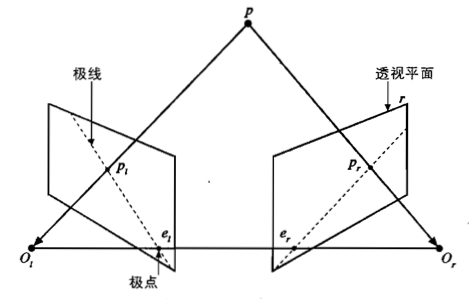
\includegraphics[width=4in]{figures/2_3_epipolar_geometry}
	\caption{对极几何示意图}\label{fig:2_3_epipolar_geometry}
\end{figure}

根据对极几何理论,给定一幅图像上的某点,其在另一幅图像上的匹配点必然位于对应的极线上,这就是“极线约束”或“对极约束”。对极约束意味着,一旦我们掌握了双目相机的对极几何,对于拍摄的两图图像间的立体匹配就从二维搜索转变为沿极线的一维搜索。应用对极约束既降低了运算量,又能排除许多可能导致虚假匹配的点。


%------------------------------------------------------------------------------------
\subsection{立体校正}
% ref: 白鹏,学习opencv.
对于平行光轴视觉模型,极线与图像坐标系的水平轴平行,而左右图像是行对齐的,从而沿极线的搜索即沿目标图像中对应行的搜索。但是平行光轴视觉模型只是一个理想模型,现实中的摄像机几乎不可能实现严格的平行对准。立体校正(stereo rectification)的目的是通过对两台摄像机的成像平面进行重投影,使它们落在同一个平面内,并且满足行对齐。Hartley\cite{hartley1999theory}、Tsai\cite{tsai1987versatile}等人提出了不同的立体校正算法,Bouguet对Tsai的算法进行了简化并开发了MATLAB摄像机标定工具箱,下面简要介绍Bouguet算法。

Bouguet算法的思想是使图像变化最小(从而使重投影畸变最小化),同时使两图的公共可视面积最大化的重投影\cite{bradski2008learning}。给定左右摄像机之间的旋转矩阵$\mathbf{R}$和平移向量$\mathbf{t}$,首先将旋转矩阵$\mathbf{R}$平分为两部分$\mathbf{r_l}$和$\mathbf{r_r}$,每个摄像机旋转一半,从而使两个成像平面平行。之后,利用极点的方向构造另一个旋转矩阵$R_{rect}$将左极点变换到无穷远处,并使极线与成像平面的水平轴平行。以主点$(c_x, c_y)$为左图像原点,指向极点的单位向量与两摄像机射影中心的平移向量方向一致:
%
\begin{equation}\label{eq:2_3_7}
\mathbf{e}_1 = \frac{\mathbf{T}}{||\mathbf{T}||}
\end{equation}

第二个向量$\mathbf{e}_2$只需要与$\mathbf{e}_1$正交。我们选择一个与新的光轴正交(即平行于图像平面)的方向,通过计算光轴方向向量$(0, 0, 1)$与$\mathbf{e}_1$的叉乘然后归一化即可得到:
%
\begin{equation}\label{eq:2_3_8}
\mathbf{e}_2 = \frac{[-T_y, T_x, 0]^T}{\sqrt{T_x^2 + T_y^2}}
\end{equation}

第三个向量需与$\mathbf{e}_1$、$\mathbf{e}_2$都正交,直接取它们的叉乘:
%
\begin{equation}\label{eq:2_3_9}
\mathbf{e}_3 = \mathbf{e}_1 \times \mathbf{e}_2
\end{equation}

从而,将左摄像机的极点变换到无穷远处的矩阵为:
%
\begin{equation}\label{eq:2_3_10}
\mathbf{R}_{rect} =
\begin{bmatrix}
(\mathbf{e}_1)^T \\ (\mathbf{e}_2)^T \\ (\mathbf{e}_3)^T
\end{bmatrix}
\end{equation}

这个旋转矩阵使左摄像机沿射影中心旋转,因此极线变为水平,极点移到无穷远处。令左右摄像机分别旋转$\mathbf{R}_l$和$\mathbf{R}_r$即可完成立体校正:
%
\begin{gather}\label{eq:2_3_11}
\mathbf{R}_l = \mathbf{R}_{rect}\mathbf{r}_l \\
\mathbf{R}_r = \mathbf{R}_{rect}\mathbf{r}_r
\end{gather}

在OpenCV中可以使用函数stereoRectify()来实现Bouguet立体校正算法,函数返回值除了$\mathbf{R}_l$和$\mathbf{R}_r$之外,还有摄像机坐标系到图像坐标系的投影矩阵$\mathbf{P}_l$、$\mathbf{P}_r$,和图像坐标系到摄像机坐标系的重投影矩阵$\mathbf{Q}$。
%
\begin{equation}\label{eq:2_3_12}
\mathbf{Q} =
\begin{bmatrix}
1 & 0 & 0 & -u_0 \\
0 & 1 & 0 & -v_0 \\
0 & 0 & 0 & \alpha_x \\
0 & 0 & -1/T_x & 0
\end{bmatrix}
\end{equation}
根据图像中某点坐标$(u, v)$和视差$d$,即可利用Q将此点投影到三维空间中:
%
\begin{equation}\label{eq:2_3_13}
\mathbf{Q}
\begin{bmatrix}
u \\ v \\ d \\ 1
\end{bmatrix}
=
\begin{bmatrix}
X \\ Y \\ Z \\ W
\end{bmatrix}
\end{equation}
三维坐标为$(X/W, Y/X, Z/W)$。


%------------------------------------------------------------------------------------
\section{本章小结}










